Nous partons de l'hypothèse que, dans un semi-conducteur, seules les deux bandes qui entourent le niveau de Fermi $\epsilon_f$ des électrons du matériau ont une influence sur ses propriétés thermodynamiques. On appelle $g_v(\epsilon)$ et $g_c(\epsilon)$ les expressions de la densité d'états dans les intervalles $\epsilon_v-\epsilon'_v$ (bande de valence) et 
$\epsilon'_c-\epsilon_c$ (bande de conduction) (voir figure ci-dessous). \`A température nulle, on admet donc que $\epsilon_v < \epsilon_f < \epsilon_c$ et on note $N=\int_{\epsilon'_v}^{\epsilon_v} g_v(\epsilon) d\epsilon$, le nombre d'électrons dans la bande de valence quand elle est entièrement remplie.


On se place désormais à une température $T$ non nulle et on note $\mu$ le potentiel chimique.


\question \'Ecrire les expressions des nombres $N_c$ et $N_v$ représentant respectivement les nombres d'électrons dans la bande de conduction et dans la bande de valence à la température $T$ et au potentiel chimique $\mu$. On introduira la distribution de Fermi-Dirac $n^F(\epsilon)$.

\question Soit $P_v=N-N_v$: on interprète ce nombre comme le nombre de trous dans la bande de valence. Expliquer. Quelle relation lie $P_v$ et $N_c$ ? En déduire l'équation formelle (avec des intégrales portant sur $g_c$ et $g_v$) permettant de calculer $\mu$.

\question \'Ecrire de même l'expression de $\Delta U$, variation d'énergie interne du semi-conducteur par rapport à son énergie au zéro absolu. 

\question Simplifier les expressions de $N_c,P_v$ et $\Delta U$ en tenant compte des inégalités respectées expérimentalement $k_B T \ll \epsilon_c - \mu $, $k_B T \ll \epsilon'_c-\epsilon_c$  et $k_B T \ll \mu - \epsilon_v$, $k_B T \ll \epsilon_v-\epsilon'_v$. 
Montrer que 
\begin{eqnarray}
N_c &=&  \int_{\epsilon_c}^{+\infty} d\epsilon \ g_c(\epsilon) \exp[-\beta(\epsilon-\mu)], \ \ P_v = \int^{\epsilon_v}_{-\infty} d\epsilon \ g_v(\epsilon) \exp[\beta(\epsilon-\mu)] \nonumber \\
\Delta U &=& \int_{\epsilon_c}^{+\infty} d\epsilon \ \epsilon \ g_c(\epsilon) \exp[-\beta(\epsilon-\mu)]-\int^{\epsilon_v}_{-\infty} d\epsilon \ \epsilon \ g_v(\epsilon) \exp[\beta(\epsilon-\mu)]. \nonumber
\end{eqnarray}


Une bonne approximation des densités d'états $g_v(\epsilon)$ et $g_c(\epsilon)$ au voisinage de $\epsilon_v$ et $\epsilon_c$ est l'approximation parabolique (voir figure): $g_v(\epsilon)=\sqrt{2R_v} \sqrt{\epsilon_v-\epsilon}$ et $g_c(\epsilon)=\sqrt{2R_c} \sqrt{\epsilon-\epsilon_c}$ où $R_v$ et $R_c$ désignent les rayons de courbure de la densité d'états  en $\epsilon_v$ et  $\epsilon_c$ respectivement. 

On donne les intégrales $\int_{0}^{+\infty} \sqrt{x} \ e^{-x} \ dx =\frac{\sqrt{\pi}}{2}$ et  $\int_{0}^{+\infty} \sqrt{x}^3 \ e^{-x} \ dx =\frac{3\sqrt{\pi}}{4}$.


\question Calculer $N_c$ en fonction  $\mu$, $T$ et des données.

\question  Calculer $P_v$ en fonction  $\mu$, $T$ et des données.

\question$^*$ Calculer $\Delta U$.  Montrer qu'en négligeant $k_B T$ devant  devant $\epsilon_v$ et $\epsilon_c$, on obtient
\begin{equation*}
\Delta U=\epsilon_c \sqrt{\frac{\pi R_c}{2}} (k_BT)^{\frac{3}{2}} \exp[-\beta(\epsilon_c-\mu)] - \epsilon_v \sqrt{\frac{\pi R_v}{2}} (k_BT)^{\frac{3}{2}} \exp[\beta(\epsilon_v-\mu)].
\end{equation*}


\question Montrer à partir des expressions de $N_c$ et $P_v$ que $\mu=\frac{\epsilon_v+\epsilon_c}{2}+\frac{k_BT}{4} \ln (\frac{R_v}{R_c})$. En déduire le niveau de Fermi $\epsilon_F$.


On se place dans l'hypothèse ou $R_v \simeq R_c \simeq R$ et on choisit le zéro de l'énergie à $\epsilon_F$. On introduit $\Delta \epsilon=\epsilon_c-\epsilon_v$.

\question Simplifier l'expression de $\Delta U$ et montrer qu'elle s'exprime sous la forme $\Delta U=\frac{\Delta \epsilon}{2} \sqrt{2\pi R}  (k_BT)^{\frac{3}{2}} \exp[-\frac{\beta \Delta \epsilon}{2}]$.

\question En déduire, en faisant les approximations légitimes,  la capacité calorifique $C$.

\question Tracer $C$ en fonction de $T$. Comment se compare cette capacité calorifique avec celle d'électrons libres dans un métal ?
\

\centerline{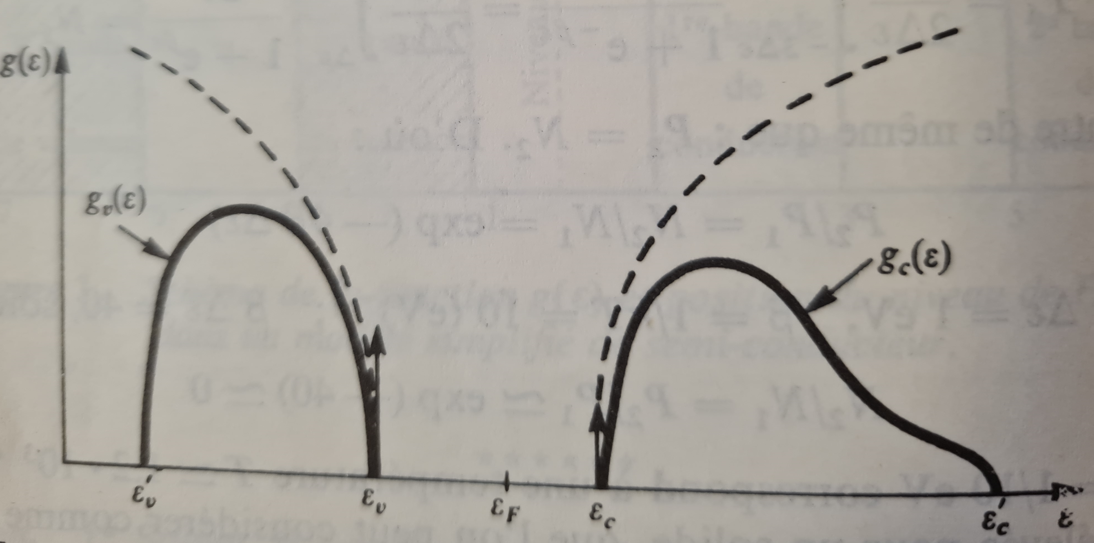
\includegraphics[height=.32\textwidth]{../Fig/Bandes}}
